\section{Tap}

Mye tap er relatert til s�kalte d�rlige omr�der, hvor det er mye rekombinasjon. Ved � karakterisere d�rlige omr�der, er det mulig � utbedre feil som det finnes kjente metoder for � unng�.

Fotoluminisensspekteret ved romtempratur er dominert av emisjon ved $h\nu_maks=1.09eV$, og et omr�de rundt $0.8eV$.  ~\cite{tarasov00}

Et eksempel p� dette er fjerning av forurensinger som jern (?) CITATION NEEDED

\subsection{Dislokasjonslinjer}

Dislokasjonslinjer er linjer som kan ses p� spektrometri spekter av eksitert lys fra pr�ven

% dislokasjonsfigur

Det er fire linjer, D1, D2, D3 og D4 som hver har sin s�regne karakteristikk.

\begin{figure}[H]
	\centering
			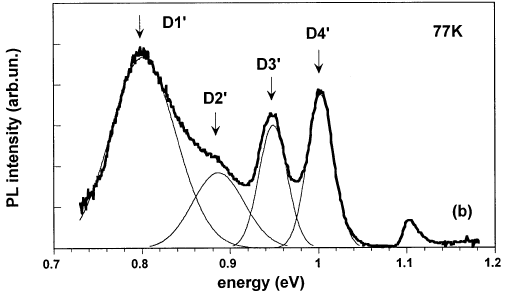
\includegraphics[width=10cm,bb=0 0 512 297]{dislokasjonslinjer_tarasov00}
		\caption{D-linjer}
	\label{fig:dislokasjonslinjer}
\end{figure}


Figur \ref{fig:dislokasjonslinjer} viser dislokasjonslinjer for multikrystallinsk silisium ved 77K. D1' er ved 0.80eV, D2' ved 0.89eV, D3' ved 0.95eV og D4' ved 1.00eV ~\cite{tarasov00}

%D1/D2 and D3/D4 belongs to different entities, based on the pl mapping.